\documentclass[border=2mm]{standalone}
\usepackage{pgfplots}
\usepackage[scaled]{helvet}
\usepackage[T1]{fontenc}
\renewcommand\familydefault{\sfdefault}
\usepackage[eulergreek]{sansmath}
\pgfplotsset{
legend style={at={(1,0.8)},anchor=east},
tick label style = {font=\sansmath\sffamily},
compat=newest}
\pgfkeys{/pgf/number format/fixed}

\begin{document}

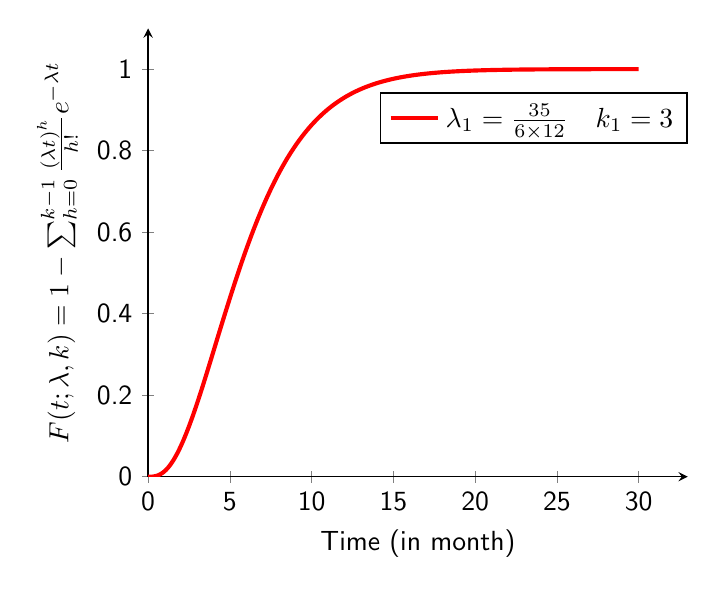
\begin{tikzpicture}
\begin{axis}[
    scaled ticks=false,
    axis lines=left,
    enlargelimits=upper,
    line width=0.5,
    legend entries={$\lambda_1=\frac{35}{6\times 12}\quad k_1=3$},
    xlabel = Time (in month),
    ylabel = {$F(t;\lambda,k)=1-\sum_{h=0}^{k-1}\frac{(\lambda t)^{h}}{h!}e^{-\lambda t}$}
]
\addplot + [smooth, mark=none, domain=0:30, samples=100, color=red, line width=1.5] {
1-exp(-35/(6*12)*x)*(1/factorial(0)+35/(6*12)*x/factorial(1)+(35/(6*12)*x)^2/factorial(2))};
\end{axis}
\end{tikzpicture}
\end{document}
